In this section, multicore architecture, shared memory programming, and Python parallel capabilities are explained in order
to give the reader a foundation in these relevant areas.

\section{Multicore architecture}

\subsection{Multicore processors}
In a typical multicore processor, several cores (which are similar to regular processors) work together in the
same system \cite[p. 44-50]{mccool_2012_structured_spppfec}. The cores consist of several \textit{functional units},
which are the core components that perform arithmetic calculations. These functional units are able to perform multiple calculation
instructions in parallel if these are not dependent on each other. This is known as \textit{instruction level parallelism}. In the multicore model,
a hierarchal cache memory architecture is used. The small, fast cache memories closest to the functional units are called \textit{registers}.
The next caches in the hierarchy are the data and instruction caches which are attached to each core. Subsequent, higher level caches that follow
these are usually an order of magnitude slower for each cache level.

\subsection{Multicore communication}
Multiple cores communicate with each other through a bus or a network \cite[p. 472-476]{herlihy_2012_art_taomprr}. Since the
means of communication between the cores is a finite resource, too much traffic may result in delays. As previously mentioned, the processors typically
have their own cache. In order to avoid unnecessary reads from the slower main memory when a cache miss is encountered for the core's own cache,
cores may read from another core that has the requested data cached. In a process called \textit{cache coherence}, shared cached values are kept up to date using one
of several protocols. The effect that these different means of communication between processors has on performance in
multicore programs should not be ignored.

\section{Parallel shared memory programming}

\subsection{Processes vs threads}
While both threads and processes represent contexts in which a program is run, they have a few differences. A thread is run inside
a process, and the threads within the process share memory and state with each other and the parent
process \cite{singh_2013_parallel_padpwprfmm}. Individual processes do not share memory with each other, and any
communication between processes must be done with message passing rather than with shared memory. Consequently, communication
between threads is generally faster than between processes.
Typically, different threads can be scheduled on different cores, which is also true for different processes.

\subsection{Data parallelism}
Data parallelism denotes code where the parallelism comes from decomposing the data and running it with the same piece of code
across several processors or computers \cite{singh_2013_parallel_padpwprfmm}. It allows scalability as number of cores and problem
sizes increase, since more parallelism can be exploited for larger datasets \cite[p. 24]{mccool_2012_structured_spppfec}.

\subsection{Task parallelism}
In task parallelism, groups of tasks that are independent are run in parallel \cite{chow_2015_pipeline_ppiaote}.
Tasks that depend on each other cannot be run in parallel, and must instead be run sequentially.
A group of tasks is embarrassingly parallel if none of the tasks in the group depend on each other.

\subsection{Scheduling}
Threads and processes are scheduled by the operating system, and the exact mechanism for choosing what to schedule when differs
between platforms and implementations \cite[p. 472]{herlihy_2012_art_taomprr}. Scheduling may imply running truly parallel
on different cores, or on the same core using time-slicing. Threads and processes may be descheduled from running temporarily for several
reasons, including issuing a time-consuming memory request.

\section{Performance models for parallel speedup}

\subsection{Amdahl's law}
Amdahl's law \cite{amdahl_2013_computer_caaal} states that:
\begin{displayquote}
The effort expended on achieving high parallel processing rates is wasted unless it is
accompanied by achievements in sequential processing rates of very nearly the same magnitude.
\end{displayquote}

Amdahl divides programs into two distinct parts: a parallelizable part and an inherently
serial part \cite[p. 13]{herlihy_2012_art_taomprr}.
If the time it takes for a single worker (for example, a process) to complete the program is $1$, Amdahl's law says
that the speedup $S$ of the program with $n$ workers with the parallel fraction of the program $p$ is:
\begin{displaymath}
  S = \frac{1}{1 - p + \frac{p}{n}}
  \label{amdahl}
\end{displaymath}

The law has the following implication: if the number of workers is infinite, the time it takes for a program to finish is still
limited by its inherently serial fraction. This is illustrated below:

\begin{displaymath}
  \lim_{n \to \infty} \frac{1}{1 - p + \frac{p}{n}} = \frac{1}{1 - p}
  \label{amdahl_lim}
\end{displaymath}

$1-p$ is the serial fraction which clearly limits the speedup of the program even with an unlimited number of processors.

\subsection{Extensions of Amdahl's law}
Che and Nguyen expand on Amdahl's law and adapts it to modern multicore processors \cite{che_2014_amdahl_alfmmp}. They find that
more factors than the number of workers affect the performance of the parallelizable part of a program, such as if the work is
more memory bound or CPU bound. In addition, they find that with core threading (such as hyperthreading), superlinear speedup of a
program is achievable and that the parallelizable part of a program is guaranteed to also yield a sequential term due to resource
contention.

Yavits et al. come to similar conclusions \cite{yavits_2014_effect_teocasoalims}. They find that it is important to minimize the
intensity of synchronization operations even in programs that are highly parallel.

\subsection{Gustafson's law}
Gustafson's law \cite{gustafson_1988_reevaluating_ral} is a result of the observation that problem sizes often grow with the
number of processors, an assumption that Amdahl's law dismisses, keeping the problem size fixed. With this premise, a program can
be run with a larger problem size in the same time as more workers are added. This view is less pessimistic than Amdahl's law, as
it implies that the impact of the serial fraction of a program becomes less significant with many workers and a large problem
size \cite[p. 61-62]{mccool_2012_structured_spppfec}.

The speedup $S$, for $n$ workers, and $s$ as the time spent in the serial part in the parallel system, is achieved by:

\begin{displaymath}
  S = n + (1-n) * s
\end{displaymath}

\subsection{Work-span model} \label{work-span}
The tasks that need to be performed in a program can be arranged to form a directed acyclic graph, where a task that
has to be completed before another precedes it in the graph. The work-span model introduces the following terms
\cite[p. 62-65]{mccool_2012_structured_spppfec}:
\begin{itemize}
  \item \textbf{Work} - The work of a program is the time it takes to complete with a single worker, and equals the total time it
    takes to complete all of the tasks. The work is denoted $T_1$.
  \item \textbf{Span} - The span of a program is the time it takes for the program to complete with an infinite number of workers.
    The span is denoted $T_\infty$.
  \item \textbf{Critical path} - The tasks that are included in the path that has the maximum number of tasks that need
    to be executed in sequence. The span is equal to the length of the critical path.
\end{itemize}

An example of a task DAG can be found in figure \ref{fig:dag_example}.

\begin{figure}[ht]
  \centering
  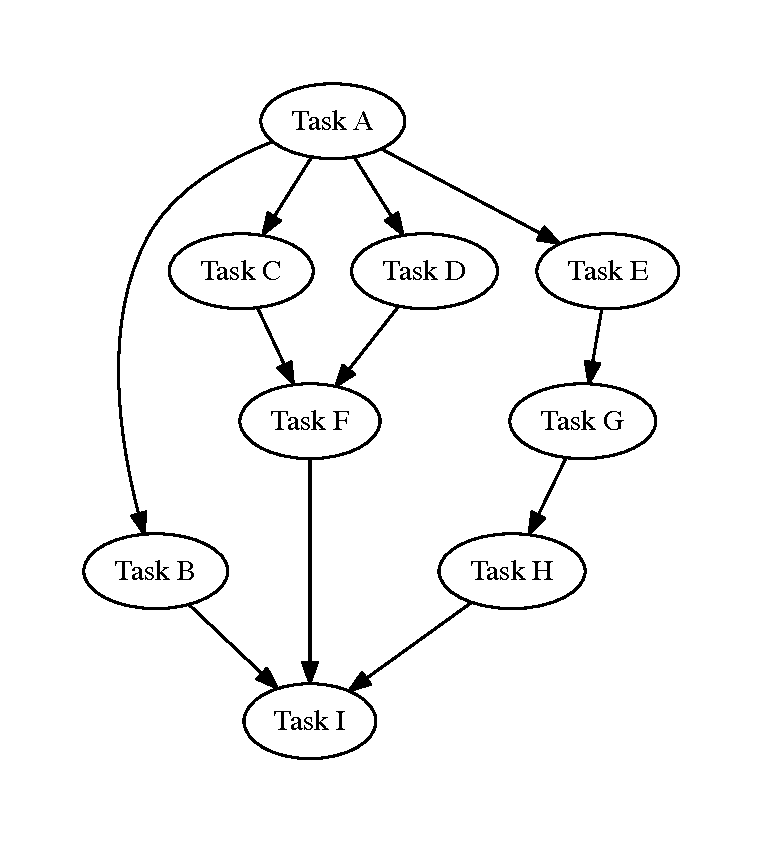
\includegraphics[width=120mm]{figures/task_dag_example.pdf}
  \caption[Example of work-span model task DAG]{An example of a task DAG used in the work-span model. Assuming each task takes
    time 1 to complete, this DAG has a \textit{work} ($T_1$) of 9 and a \textit{span} ($T_\infty$) of 5. The upper bound for
    parallel speedup for this dag is $\frac{9}{5} = 1.8$.}
  \label{fig:dag_example}
\end{figure}

In the work-span model, the following bound on the speedup $S$ holds:

\begin{displaymath}
  S \leq \frac{T_1}{T_\infty}
\end{displaymath}

With $n$ workers and running time $T_n$, the following speedup condition can be derived:
\begin{displaymath}
  S = \frac{T_1}{T_n} \approx P \text{ if } \frac{T_1}{T_\infty} \gg P
\end{displaymath}

In essence, this means that linear speedup can be achieved under the condition that the work divided by the span is significantly
larger than the number of workers.

The work-span model implies that increasing the work in an excessive manner when parallelizing may result in a disappointing
outcome. It also implies that the span of the program should be kept as small as possible in order to utilize parallelization as
much as possible.

\section{Python performance and parallel capabilities}
There are several implementations of the Python language. This section will focus on CPython, the canonical and most popular
Python implementation \cite{pythonimplementations_ppw}. This thesis uses Python 2.7.

\subsection{Performance}
The general performance of CPython is slower than other popular languages such as C and Java for several
reasons \cite{barany_2014_python_pipd}. Overhead is introduced due to the fact that all operations need to dispatched dynamically,
and accessing data demands the dereferencing of a pointer to a heap data structure. Also, the fact that late binding is employed
for function calls, the automatic memory memory management in the form of reference counting, and the boxing and unboxing of
methods contribute to the at times poor performance.

\subsection{The GIL, Global Interpreter Lock}
In order to simplify the implementation and to avoid concurrency related bugs in the CPython interpreter,
a mechanism called the Global Interpreter Lock - or the GIL - is employed  \cite{palach_2014_parallel_ppwp}.
The GIL locks the entire CPython interpreter, making it impossible for multiple Python threads to make progress at
the same time, thereby removing the benefits of parallel CPU bound calculations
\cite{glossary_gp2d}. When an I/O operation is started from Python, the GIL is released.
Efforts to remove the GIL have been made, but have as of yet been unsuccessful.

\subsection{Threading}
The Python \code{threading} module provides a multitude of utilities for concurrent programming, such as an object abstraction of
threads, locks, semaphores, and condition objects \cite{16_1thtip2d}. When using the \code{threading} module in CPython, the GIL is in
effect, disallowing true parallelism and hampering efficient use of multicore machines. When performing I/O bound operations, the
\code{threading} module can be used to improve performance; at times significantly \cite[p. 121-124]{slatkin_2015_effective_ep5swtwbp}

\subsection{Multiprocessing}
The \code{multiprocessing} module has a similar API to the \code{threading} module, but avoids the negative effects of the GIL by spawning
separate processes instead of user threads. This works since the processes have separate GILs, which do not affect each other and
enables the processes to utilize true parallelism \cite{slatkin_2015_effective_ep5swtwbp}. The processes are represented by the \code{multiprocessing.Process} class.

The \code{multiprocessing} module provides mechanisms for performing IPC.
In order for the data to be transferred between processes, it needs to be serializable through the use of the Python \code{pickle}
module \cite[p. 143]{slatkin_2015_effective_ep5swtwbp}. When transferring data, it is serialized, sent to another process through
a local socket, and then deserialized. These operations, in conjunction with the creation of the processes, gives the
\code{multiprocessing} module a high overhead when communicating between processes.

The two main facilities that the \code{multiprocessing} module provides for IPC are \cite{palach_2014_parallel_ppwp}:
\begin{itemize}
  \item \code{multiprocessing.Pipe}, which serves as a way for two processes to communicate using the operations \code{send()}
    and \code{recv()} (receive). The pipe is represented by two connection objects which correspond to each end of the pipe.
    See figure \ref{fig:code_pipe_example} for an example.
  \item \code{multiprocessing.Queue}, which closely mimics the behaviour and API of the standard Python \code{queue.Queue}, but
    can be used by several processes at the same time without concurrency issues. This \code{multiprocessing} queue internally
    synchronizes access by multiple processes using locks, and uses a \emph{feeder thread} to transfer data to other processes.
    See figure \ref{fig:code_queue_example} for an example.
\end{itemize}

In addition to the parallel programming utilities mentioned above, the \code{multiprocessing} module provides the \code{Pool} abstraction
for specifying a number of workers as well as several ways of assigning functions for the workers to be performed in parallel. For
example, a programmer can use \code{Pool.map} to make the workers in the pool execute a specified function on each element in a
collection.
See figure \ref{fig:code_pool_example} for an example.

\begin{figure}[ht]
  \centering
  \pythonexternal{code_examples/pipe_example.py}
  \caption{\code{multiprocessing.Pipe} example}
  \label{fig:code_pipe_example}
\end{figure}

\begin{figure}[ht]
  \centering
  \pythonexternal{code_examples/queue_example.py}
  \caption{\code{multiprocessing.Queue} example}
  \label{fig:code_queue_example}
\end{figure}

\begin{figure}[ht]
  \centering
  \pythonexternal{code_examples/pool_example.py}
  \caption{\code{multiprocessing.Pool} example}
  \label{fig:code_pool_example}
\end{figure}

